%%%%%%%%%%%%%%%%%%%%%%%%%%%%%%%%%%%%%%STARt PREAMBLE
\documentclass{article}

%Required: You must have these
\usepackage{Sweave}
\usepackage{graphicx}
\usepackage{tabularx}
\usepackage{hyperref}
\usepackage{natbib}
\usepackage{pdflscape}
\usepackage{array}
\usepackage{authblk}
\usepackage{gensymb}
\usepackage{amsmath}
%\usepackage[backend=bibtex]{biblatex}
%Strongly recommended
 %put your figures in one place
%\SweaveOpts{prefix.string=figures/, eps=FALSE} 
%you'll want these for pretty captioning
\usepackage[small]{caption}

\setkeys{Gin}{width=0.8\textwidth} %make the figs 50 perc textwidth
\setlength{\captionmargin}{30pt}
\setlength{\abovecaptionskip}{10pt}
\setlength{\belowcaptionskip}{10pt}
% manual for caption http://www.dd.chalmers.se/latex/Docs/PDF/caption.pdf

%Optional: I like to muck with my margins and spacing in ways that LaTeX frowns on
%Here's how to do that
\topmargin -1.5cm  
\oddsidemargin -0.04cm 
\evensidemargin -0.04cm % same as oddsidemargin but for left-hand pages
\textwidth 16.59cm
\textheight 21.94cm 
%\pagestyle{empty}  % Uncomment if don't want page numbers
\parskip 7.2pt   % sets spacing between paragraphs
%\renewcommand{\baselinestretch}{1.5} 	% Uncomment for 1.5 spacing between lines
\parindent 0pt% sets leading space for paragraphs
\usepackage{setspace}
%\doublespacing
\renewcommand{\baselinestretch}{1}
\usepackage{lineno}
 
%%%%%%%%%%%%%%%%%%%%%%%%%%%%%%%%%%%%%%END PREAMBLE 

%Start of the document
\begin{document}

%\SweaveOpts{concordance=FALSE}
\Sconcordance{concordance:bayes4cons_doc.tex:bayes4cons_doc.Rnw:1 310 1}


\bibliographystyle{bibstyles/amnat.bst}
\title{Adaptive conservation science using Bayesian methods} 
\author[1,a]{A.K. Ettinger}
\author[2]{Harold N. Eyster}
\author[3]{Hanna Jackson}
\author[4,5]{D. Loughnan}
\author[6]{M. Auger-M\'eth\'e}
\author[3]{Leithen M'Gonigle}
\author[7]{X. Wang}
\author[7]{E.M. Wolkovich}


\affil[1]{The Nature Conservancy, Seattle, Washington, USA}
\affil[2]{The Nature Conservancy, Boulder, Colorado, USA}
\affil[4]{Department of Zoology, University of British Columbia, Vancouver, British Columbia, Canada}
\affil[5]{Hakai Institute, Campbell River, British Columbia, Canada}
\affil[6]{Department of Statistics and Institute for the Oceans and Fisheries The University of British Columbia}
\affil[3]{SFU}
\affil[7]{UBC Forestry}


\affil[a]{Corresponding author; email: ailene.ettinger@tnc.org; mailing address: 74 Wall Street. Seattle, WA 98121, USA }

\date{\today}
\maketitle 
\textbf{Author contributions}: All authors conceived of this manuscript, which began through conversations at a Bayesian Generative Modelling Symposium at University of British Columbia in 2024; AKE led the writing of the manuscript, all authors contributed portions of text and revised the manuscript.

\textbf{Data Accessibility} 

\textbf{Running title} 

\textbf{Key words} 


\textbf{Paper type} \textit{Perspective} in \href{https://conbio.onlinelibrary.wiley.com/hub/journal/1755263x/homepage/forauthors.html#ATypes}{Conservation Letters} (3,000 words). Back-up/next journal to submit to is \href{https://conbio.onlinelibrary.wiley.com/hub/journal/25784854/homepage/author-guidelines}{Conservation Science and Practice} or \href{https://www.sciencedirect.com/journal/environmental-science-and-policy/publish/guide-for-authors}{Environmental Science and Policy}

\textbf{Focal Audience} Conservation biologists and other scientists who contribute to or would like to influence conservation and environmental policy (e.g., IPCC, IUCN)

%%%%%%%%%%%%%%%%%%%%%%%%%%%%%%%%%%%%%%%%%%%%%%%%%%%

%%%%%%%%%%%%%%%%%%%%%%%%%%%%%%%%%%%%%%%%%%%%%%%%%%%

%\linenumbers

\section*{Abstract} 


%reread with concept of posterior in mind- 
\newpage
\section* {Introduction}

Conservation science is an interdisciplinary field focused on protecting and managing biodiversity and natural ecosystems, both to sustain long-term health of nature and to benefit human well-being \citep{kareiva2012conservation}. At its start, conservation science often focused on spatial analyses to identify priority areas to establish parks and preserves intended to protect threatened species and communities \citep{bocking2020science}. Climate change has layered additional challenges to preserve establishment as a conservation strategy, since protecting today's habitats from development or other land use changes does not guarantee suitable conditions in a future warmer world. In addition climate change both affects biodiversity \citep[e.g., by causing extinctions][]{urban2024climate} and is affected by biodiversity conservation \citep[e.g., nature-based climate solutions or `natural climate solutions'][]{griscom2017natural}. Integrating approaches to bolster adaptation and resilience to climate change, as well as greenhouse gas mitigation, are critical components of planning and implementing conservation in the era of climate change.

\par The need for robust and usable conservation science under climate change is necessary at scales ranging from local to global. For example, preserve managers seek guidance about how to best steward natural resources for climate resilience \citep{Nadeau2015}, and  international climate policymakers rely on scientific data and publications for systematic observation of climate systems and impacts to people \cite{ipcc2007}. As 'crisis discipline' practitioners, conservation biologists, like medical doctors, often need to act rapidly and without complete knowledge \citep{soule1985conservation}. Rather relying only on personal experience or word of mouth in such situations, as was frequently done in the past, medical and conservation practitioners alike increasingly rely on evidence that has been systematically accumulated through meta-analyses and other syntheses \citep{kareiva2012conservation}. Developing the evidence base for urgent climate and biodiversity problems often requires synthesizing multiple data sources and incomplete datasets, given the complex ecological systems in which many conservation science problems are grounded. A critical part of building this evidence base is ensuring reproducibility and transparency, including clear communication of uncertainty \citep{ellis2024principles,ipcc2007}. 

\par Addressing conservation problems requires information beyond ecology; social, cultural, political and economic data, in addition to biological and physical information, are often needed to provide the evidence base upon which decisions can be made. Focal populations of threatened species are often small, and ecological and social data are often non-normal, `unbalanced' and nested within hierarchical or non-hierarchical groupings that are non-independent (e.g., species or other groupings related to evolutionary history/genetics, spatial clustering such as plots or sites, or temporal clustering such as day or year). These qualities challenge many traditional, commonly used statistical approaches (e.g., analysis of variance). Further, conservation evidence comes in many forms, including from quantitative studies, community knowledge (add ref), expert knowledge (add ref), indigenous knowledge \citep[e.g.,][]{gryba2023indigenous}, and others. Conservation decision-making requires integrating these multiple sources of information to provide an evidence base for decision-making \citep{stern2022interweaving}. 

\par Bayesian data analysis provides a framework and approaches that support these needs of conservation science in the 21st century. Bayesian approaches facilitate synthesis of multiple sources of data to update probabilities of focal outcomes of interest after examining new data (i.e., a `prior', which is a probability distribution that represents the modeler's pre-existing beliefs or knowledge about a model parameter before any new data is considered, see Box 1). Bayesian methods are well-suited to decision making, as they move beyond strict null-hypothesis testing to provide a quantitative measure of the probability of a hypothesis being true given the available data. Some fields within conservation biology and natural resource management have adopted Bayesian methods (e.g., wildlife mark and recapture models or occupancy models \citep{Kery2011}, fisheries \citep{Doll2018}), but they have yet to be widely used across conservation biology. (could add "and have not been integrated into policy and management.")

\subsection*{Aim} Here,  we highlight features of Bayesian approaches that are well-suited to conservation science for practitioners who may be unfamiliar with Bayesian methods. We first review some benefits of using Bayesian methods to address conservation science questions, focusing on three key features: the iterative workflow process, flexible modelling frameworks, and integration of uncertainty. We also share resources that we hope will make Bayesian methods more approachable to those who have not used them before, including example code and analyses through three case studies relevant to current conservation problems, and a list of resources to get started with these methods. Even if readers do not use Bayesian approaches themselves, we hope they will better understand why and how they can be beneficial. We hope to accelerate more widespread adoption of and comfort with Bayesian data analytical approaches, as the time is right for integration into conservation science, policy, and practice. 

\section* {Benefits of Bayesian Modelling for Conservation Science}
\subsection*{Iterative workflows for adaptive management}
\par As conservation scientists implement interventions in variable and dynamic ecosystems that often exhibit unexpected behaviors \citep{Levin2012,Gross2013}, the practice of adaptive management has become common \citep{holling1978adaptive} (Fig. \ref{fig:workflow}). Cycles of adaptive management include stages of \underline{assessing} threats and conservation goals, \underline{planning} strategies, implementation, and monitoring, \underline{implementing} those plans, \underline{analyzing} results of initial implementation, \underline{adapting} implementation based on these analyses, and \underline{sharing learning} from the process. This cycle of iteration continues until the end of the project, ideally when conservation goals are met, and the intention is for this evidence-based approach to lead to improved conservation outcomes (https://www.conservationbydesign.org/).

\par Bayesian modeling's workflows also follow an iterative process, but provide opportunities to integrate model development much earlier into the adaptive management cycle. Major training resources for adaptive management often place data analysis late in the cycle, as visually represented in the Conservation by Design diagram shown in (Fig. \ref{fig:workflow}). This is a dangerous practice because potential problems with study design, data collection practices, or other issues may not be identified until after it is too late to make changes. We believe that integrating the modelling workflow throughout the cycle would lead to valuable insights earlier in process, result in more robust conservation science and, perhaps, then better outcomes after implementation. Model development can occur in the \underline{assessing} stage, and be tested with simulated data in the \underline{planning} stage. Data collection occurs as part of monitoring during the \underline{implementing} stage and then models are run with empirical data as part of the \underline{analyzing} stage. Model checking and revising occurs during \underline{adapting} stages and then \underline{sharing learning} about modelling as well as conservation implementation occurs in parallel.  

\subsection*{Flexible frameworks for complex data}
%dlOct17: I think this could be where we integrate case study 3, as an illustration of how expert knowledge can help make better priors and predictions
\par Bayesian modelling approaches are well-suited to address the complexity and incomplete nature of many conservation datasets, given their flexibility and power to provide robust estimates under a wide range of conditions (e.g., Case Study 1). Bayesian models can be specified to include a wide range of data distributions via ready-to-use packages in programs like R (e.g., 'brms'), and expanded to infinite  model specifications when the user codes them by hand. Multiple sources and types of data can be amalgamated into Bayesian Belief Networks \citep{marcot2001using,newton2007bayesian}, and extant information can be used to inform `prior distributions' used in Bayesian modelling \citep{o2008informed,mcneish2016using}. (For more on what `prior distributions' or `priors' are, see Box 1.)
Bayesian methods are also well-suited to accommodate the small population sizes that are often a focus of conservation because they are at high risk of extinction \citep{stinchcombe2002influence}. Because Bayesian methods do not rely on asymptotic behavior (as frequentist statistics due \citep{mcneish2016using}), they are better able to accommodate small sample sizes.
\par The flexibility of Bayesian methods is also beneficial and well-suited to conservation planning because they move beyond 'null hypothesis' frameworks and a focus on p-values to facilitate comparison of support for a variety of hypotheses or interventions \citep{Zyl2018}. Null hypothesis significance testing and conventions of rejecting the null hypothesis when p $<0.05$ have long been dominant in conservation biology, as in ecology and related biological fields \citep[e.g., ecotoxicaology][]{erickson2020moving}. P-value-focused conventions are becoming less prevalent, but many biologists are unsure of alternative ways to analyse and interpret their data \citep{halsey2019reign}. Bayesian approaches and workflows offer an alternative framework, facilitating, for example, assessments of which interventions will result in greater conservation gains \citep{prato2005bayesian}, whether the current versus alternative management practices produce similar results \citep{gallistel2009importance}, and whether a population has passed a particular threshold, such as declining `rapidly' versus `moderately', as defined by a particular probability \citep{brooks2008quantifying}. The flexibility and power of Bayesian modelling require training to implement, as well as thoughtful specification and careful interpretation. We believe this is not unique to Bayesian modelling; rather it is applicable to all statistical tools and approaches.
%dlOct18 Above is where I would introduce case study 1 to illustrate how p-values vs Bayesian can lead to different conclusions 

%\subsection*{Moving beyond null hypothesis testing and $\alpha <0.05$ } %Yet frequentist statistical frameworks rarely provide information necessary to adequately inform adaptive management \citep{prato2005bayesian}.  Specifically, frequentist statistics' incapacity to compare support for a variety of hypotheses \citep[including a `null' hypothesis;][]{Zyl2018} prevents this method from informing what interventions will most likely bring about conservation gains \citep{prato2005bayesian}. For example, in its submission process, leading conservation journal \textit{Conservation Biology} requires that authors recognize that, `8. ensured you have not misinterpreted statistical nonsignificance as no effect if a frequentist approach was used (absence of evidence is not evidence of absence)?'
\subsection*{Quantifying and propagating uncertainty} 
\par  Many conservation problems require integrating and propagating uncertainty across multiple datasets, multiple sources and/or multiple modeling steps (see Case Study 2). Bayesian approaches enable straightforward quantification and  propagation of  uncertainty \citep[e.g.,][]{stern2022interweaving, draper1995assessment,gilbert2023propagating} that is intuitive (e.g., posteriors of estimates from different sources can be added and averaged yielding new means, standard deviations etc.). This makes it easier for non-statistician colleagues and decision-makers to engage in the modeling step (cite our new adaptive mgmt figure?) \citep{fornacon2021bayesian}. This is also helpful for some conservation problems that can require analyses for which frequentist statistics are unable to compute the associated uncertainties \citep{bolker2009a,bates2006r}.  \cite{Eyster2022} provide an example of applying Bayesian methods to estimate the abundance of birds in different types of management landscapes (traditional agriculture, perennial polycultures) and propagating the uncertainty associated with those abundances into a downstream analysis to test whether the bird communities in the alternative perennial polyculture landscape are maintained as an ecological sink. 

%old version of above paragraph: \par Moreover, Bayesian methods enable uncertainty to be propagated through multiple analyses, ensuring that end results represent the full uncertainty of the process under study. \citep{draper1995assessment,gilbert2023propagating,Eyster2022,Saunders2019}. 
%dlOct18: This is a really cool example, I also think this could be a good point to introduce our 2nd case study and use it as the example of how uncertainty is propagated in Bayesian methods.
%emw1Nov: I agree with Deirdre, if this could be added as a case study figure and/or replace a case study it would be great! This would then mean this paragraph becomes one sentence that cites the figure and fits nicely into the last paragraph. The case study does not need code, it would be nice if it were just a conceptual figure IMHO.
%From Lizzie: IUCN `Rules of Procedure’ (download here) are pretty vague on uncertainty (and have two types at least: Uncertainty in the data and uncertainty in taxonomic). I think our relevant interest in the IUCN goal is to get to ‘Direction of current population trend (stable, increasing, decreasing, unknown)’ and there are actually are some papers about what to do about uncertainty in this for the IUCN. One well-cited one is: Making Consistent IUCN Classifications under Uncertainty (2000, JSTOR link), which I think basically advocated fuzzy numbers (but I did not read closely; this paper seems to have led to the RAMAS software). There’s a literature from this citation including a Bayesian network (Use of a Bayesian network for Red Listing under uncertainty, 2010) that someone could dig into a little more? See also: JARA: ‘Just Another Red-List Assessment’

\section* {Increasing use of Bayesian approaches}
\par Though Bayesian methods are increasing, they are not yet standard, widely used approaches that are well-integrated into national or global systems of conservation and climate science, policy and practice (e.g., IPCC, IUCN). For example, IPCC-described methods for uncertainty propagation do not include Bayesian approaches \citep{ipcc2007}, though these approaches would offer straightforward implementation (e.g., for propagating uncertainty, Case Study 2). 

\par Uptake and use of Bayesian methods is also highly variable across disciplines, suggesting opportunities to test their utility in fields where they are less used. For example, fisheries and wildlife biology generally used Bayesian approach more often than forestry and plant ecology (Fig. \ref{fig:consbaystrend}). Often this is because certain modeling approaches that are most easily fit through Bayesian approaches have become standard in these fields. For example, mark-and-capture models within wildlife biology \citep[e.g.,][]{royle2013spatial,calvert2009hierarchical},  fisheries stock assessment approaches that integrate over different data to give the best estimates \citep[e.g.,][]{punt1997fisheries}. This suggests that once fields begin to use Bayesian approaches they appreciate the advantages---models that better match their data and biology and allow them to better understand their uncertainty---and these approaches become more widespread and standard. We see opportunities for more widespread use to achieve these same benefits in other disciplines. For example, Bayesian models in plant ecology could incorporate observation and process models---similar to what has been used in wildlife biology---to help separate which trends are due to shifts in monitoring effort versus shifts in biology \citep[][]{pearse2017statistical}.


\par Within the general increase in use of Bayesian methods, there appears to be notable variation by discipline. For example, there may be more widespread use in fisheries and wildlife biology, and less in forestry and plant ecology (Fig. \ref{fig:consbaystrend}). This may reflect adoption of particular model types within disciplines, such as mark-and-capture studies within wildlife biology \citep[e.g.,][]{royle2013spatial,calvert2009hierarchical}, or high-demand applications within natural resource management that can be met by Bayesian modelling, such as fisheries stock assessment \citep[e.g.,][]{punt1997fisheries}. We see opportunities for more widespread use within disciplines that do not appear to have  taken up Bayesian approaches as rapidly. For example, within plant ecology, incorporation of Bayesian models that incorporate observation and process models, similar to what has been used in wildlife biology, may allow for better separation of trends due to shifts in monitoring effort versus shifts in biology \citep[][]{pearse2017statistical}.


\section* {A future with more widespread use of Bayesian modelling in Conservation}
\par The urgency of conservation problems and complexity of  ecological systems requires flexible, powerful modelling approaches, a challenge with which many traditional approaches (e.g., $t$-tests) struggle. Integrating Bayesian modelling approaches in conservation training and practice could help meet this challenge. If conservation and ecology students, across undergraduate and graduate levels, received analytical training that included strong foundations in Bayesian statistics they could more easily integrate many of the data, modeling, and uncertainty challenges into adaptive management (cite Fig). We argue the time to make this change is now, as Bayesian modelling has become easier given increased access to computational resources and training (see, e.g., Resources to Get Started). Further, given the utility and increasing use of Bayesian approaches (Fig. \ref{fig:consbaystrend}), we believe that the IPCC, IUCN and other global institutions should include Bayesian approaches as accepted options. These flexible and powerful approaches can help us develop more robust understanding of complex ecological systems, and facilitate fuller use of the data we have to address urgent conservation problems under climate change.

\par Add this somewhere:
Ecology and conservation science have become more quantitative and data-driven fields in recent decades, and use of Bayesian approaches appears to be increasing \citep{anderson2021trends}. The rise in Bayesian approaches likely reflects an acknowledgement of their utility, given the benefits they offer, including those we mention here. 

%emw1Nov: I edited the above paragraph and deleted out the below which I think should go above when we first introduce the IPCC
%  and as biological feedback get more integrated into the climate/biophysical analyses that dominated early IPCC work


\section* {Case Studies}
\subsection*{Case Study 1: Robust estimates of trends in species or populations of concern}
\par In some cases, Bayesian approaches can lead to importantly different conclusions than common Fisherian approaches, such as null hypothesis testing citep{wade2000bayesian}. Consider, for example, sampling five populations of a species across its range---from north to south---to monitor for changes in the population size with climate change. After collecting data for ten years, a traditional null hypothesis testing approach to analyzing the data, using the commonly used significance level ($\alpha$) of 0.05 would find changes in only two of the populations---the furthest north population, which appears to be increasing, and the second furthest north population, also increasing. The three other populations are not significantly changing under this approach (Fig. \ref{fig:nht} left). In contrast, a Bayesian approach (using weakly informative priors centered at zero, all code provided in supplement) would likely focus on the posteriors, where small differences in the variance do not appear so different  (Fig. \ref{fig:nht} right). Here, a clear trend emerges where trends in population correlate with position in range---with the most northern population increasing the most and the most southern population decreasing the most. This pattern across the range is the type predicted by climate change and may be missed with a classic Fisherian approach (combining null hypothesis testing with threshold values for `significance'), leading to potential very difference conservation and management decisions. % EMW says: We could also add (1) more details on the simulations (the variance in the underlying model increases going from north to south, which is expected for smaller population sizes), (2) point out 10 years is often more years than we have; though I think there is enough text already. 


\subsection*{Case Study 2: Incorporating and propagating uncertainty}

\par One major approach that integrates biodiversity conservation and climate change mitigation is `natural climate solutions' (NCS) \citep{ellis2024principles}, also called nature-based climate solutions. NCS are intentional human actions (or `NCS pathways') that protect, restore, and improve management of forests, wetlands, grasslands, oceans, and agricultural lands to mitigate climate change \citep{griscom2017natural}. Estimating mitigation potential of NCS involves multiple sources of uncertainty, many of which are not incorporated in commonly used approaches. We simulate flux data from a field study quantifying methane fluxes in peatlands with and without grazing in Ecuador \citep{sanchez2017carbon} to show how Bayesian approaches can be used to propagate uncertainty from area, as well as fluces,in a straightforward way (Fig.\ref{fig:ncs}). 

\subsection*{Case Study 3: State-space model and priors example}
%emw1Nov: I wonder if this case study would work better as a conceptual figure (boxes, arrows) to just explain state space models, which we actually discuss a bit. I feel like the current example is great, but it's a bit more tricky to grasp and not critical for readers of the paper, whereas helping them understand observation versus process models is ... if we did this it could be a two-panel figure with Harold's example of propagating uncertainty on one side and Marie's example of combining observation and process models on the other. More conceptual figures would also hive with the quick and upbeat tone of the current ms (which I like!).
\par We demonstrate use of priors via a population model, described in Auger-Methe et al 2021 and based on Jamieson and Brooks (2004) and Dennis and Taper (1994). This is a simple population model with density dependence, made up of process and observation components, as described at \href{https://github.com/AileneKane/bayes4cons/blob/main/analyses/SSM.Rmd}{https://github.com/AileneKane/bayes4cons/blob/main/analyses/SSM.Rmd}

\par In this scenario, we have re-introduced 10 adult females and some 10 adult males from an extirpated species in 2003 in a conservation area, and we are monitoring their growth for the past 20 years to see if they have reached carrying capacity and what is that carrying capacity.

\par This is a species that has a long life span (e.g. 20+ years) and creates long term pairs  that can produce maximum 2 offspring when in good conditions, and therefore could be able to almost double in size ever year. Here the conservation area does not allow the animal to fulfill it's full growth ($\beta_0 = 1.3$). From a repeated assessments of the efficiency of the line transect in early years, when all of the re-introduce animals were individually marked, we know that we can miss many individuals and have estimated the $\sigma_o = 10$.

\par As for most population of this species the birth rate, which is the main source of biological stochasticity, vary by less than 5%.

\par When we fit the model with vague priors, there are many warnings, indicating the model is problematic. However, when we use knowledge gained from previous studies of species' biology to inform priors, we are able to fit models.
%DLJuly30: I think case study 3 makes the most sense as a vignette---there is a lot of ecology for the background and to explain what the priors are. As a reader, I would want an explanation for what the warnings mean and how they inform the process. I also think if our goal is to emphasize prior selection, we need to be more explicit in explaining what the vague priors are and what kinds of knowledge was needed to develop informative priors.

\par 
\section* {Box 1: Defining Bayesian Analysis (i.e., Inference and Workflow)}

Bayesian methods allow us to combine prior knowledge of a system with available data to quantitatively measure the probability of a model or hypothesis being true. A Bayesian model treats parameters as random variables for which a known probability distribution is defined based on prior knowledge of the parameter uncertainty. By incorporating expert knowledge of ecological processes or species natural history, this modelling approach allows the development of bespoke and uniquely formulated models for any given data-generating process.\\

At the foundation of this statistical approach is the use of Bayes' Theorem (eqn 1). This theorem consists of three components: a prior distribution (A) %P(A)? here and in equation below
as defined using data from previous experiments, expert opinions, or literature, and a likelihood function ($f(B|A)$), which are combined to estimate the probability distributions for each parameter (\emph{P}(A|B)). \\
\begin{align}
 \emph{P}(A|B) = \frac{f(B|A)(A)}{P(B)}
 \end{align}
 %From MAM: You will also have to define A. Also, note that you could use H for A and Y for B. Then you'd be in line with the Ellison paper notation ;)
Since the results of Bayesian methods are probabilistic, they allow us to make stronger inferences based on a model's predicted uncertainty. As new data is collected or inferences made, we can revise our model priors and iteratively improve our understanding of the data-generating processes that underlie ecological systems. Model estimates can be further used to perform simulations and more robustly forecast changes under future conditions. 

Our aim here is not to provide an exhaustive explanation of Bayesian statistics, but to provide a brief introduction of core components of a Bayesian model and their relationships. For an in depth discussion of Bayesian statistics, we recommend the \emph{Gentle Introduction to Bayesain statistics} by \cite{van2014gentle}, \emph{Bayesian model selection for ecologists} by \cite{hooten2015guide}, and \emph{Bayesian Inference for ecologists} by \cite{elis2004}. For further discussion of prior selection for ecological models, see \cite{banner2020priors}.
% Inference in frequentist statistics can take many forms, but here we focus on the most dominant incarnation, which entails testing the significance of a null hypothesis given data, measured with a p-value \citep{Zyl2018}. Bayesian analysis can be formulated in a variety of different ways (Lee, 2011). Frequentist methods have previously dominated ecological analyses.
% \begin{itemize}
% \item Frequentist methods—that rely on the frequency of an event's occurrence in a sample dataset given a particular hypothesis to estimate its probability.
% \item Bayesian methods—provides a quantitative measure of the probability that a hypothesis is true using available data
% \item Frequentist methods—only make use of the sample data
% \item Bayesian methods—bring prior knowledge together with the sample data
% \item Frequentist methods—parameters  are considered to be estimates of fixed
% \item Bayesian methods—model parameters are treated as random variables
% \item Frequentist methods—cares about p-value, significance, confidence interval
% \item Bayesian methods—cares about credible interval, prior, posterior
% \end{itemize}
% Bayesian methods use Bayes' Theorem (eqn. 1) to combine our prior knowledge of a system with the available data to estimate the probability of an event. 
% Does not assume that parameters are the fixed or true quantities
% Since inferences are probabilistic—can perform simulations using the density distributions of their parameters and make stronger inference of models predictive uncertainty
% P(A|B) = f(B|A)(A)/P(B)
% \par Three components:
% \begin{itemize}
% \item Posterior distribution (P(A|B)): used to update the prior using the likelihood
% \item Likelihood ( f(B|A)): function of how likely te response variable is given the data
% \item Prior ((A)): pre-existing information about the hypothesis—data from pilot studies or previous experiments, knowledge from experts or the literature—reflect the uncertainty within the system
% \end{itemize}
% \par Bayesian modeling is an iterative process: analyses may start with insufficient knowledge and data but use experiments to inform priors, and uses model checking to test key assumptions and our understanding of the data generating process.
% \par General Bayesian workflow (Fig. \ref{fig:workflow})
% \begin{itemize}
% \item Simulate data based on priors and initial model specification 
% \item Collect data
% \item Model construction and testing
% \item Prior predictive checks→Fit model to data
% \item Posterior predictive checks
% \item Summarize posteriors
% \item Report results to targeted audiences
% \end{itemize}
% 


% \section* {Box 2: Resources to Get Started}
% \underline{Priors}
% \par Default priors. Chosen without critical thought or evaluation. Fear of being too subjective. Defending prior choice promotes good statistical inference
% \par Resources on priors: 
% 
% \begin{itemize}
% \item Banner et al. 2020 https://besjournals.onlinelibrary.wiley.com/doi/full/10.1111/2041-210X.13407 
% \end{itemize}
% 
% \par Other resources:
% \begin{itemize}
% \item A guide to Bayesian model checking for ecologists \citep{conn2018guide}
% \item Gentle Introduction to Bayesian statistics \citep{van2014gentle}
% \href{https://www.ncbi.nlm.nih.gov/pmc/articles/PMC4158865/}{https://www.ncbi.nlm.nih.gov/pmc/articles/PMC4158865/}
% \item Bayesian model selection for ecologists. \citep{hooten2015guide}
%  \href{https://doi.org/10.1890/14-0661.1}{https://doi.org/10.1890/14-0661.1}
% \item Bayesian Inference for ecologists. \citep{elis2004}
% \item Why becoming Bayesian? \citep{clark2005environmental}
%  \href{https://doi.org/10.1111/j.1461-0248.2004.00702.x}{https://doi.org/10.1111/j.1461-0248.2004.00702.x}
% \item Bayesian Workflow \citep{gelman2020bayesia}
% 
% \end{itemize}
%xwNov1: I think maybe we can make this box more informative by relating resources we included here to the sections we have in the paper. 


\bibliography{conslib.bib}

\section* {Figures}
 \begin{figure}[h]
\centering
 
  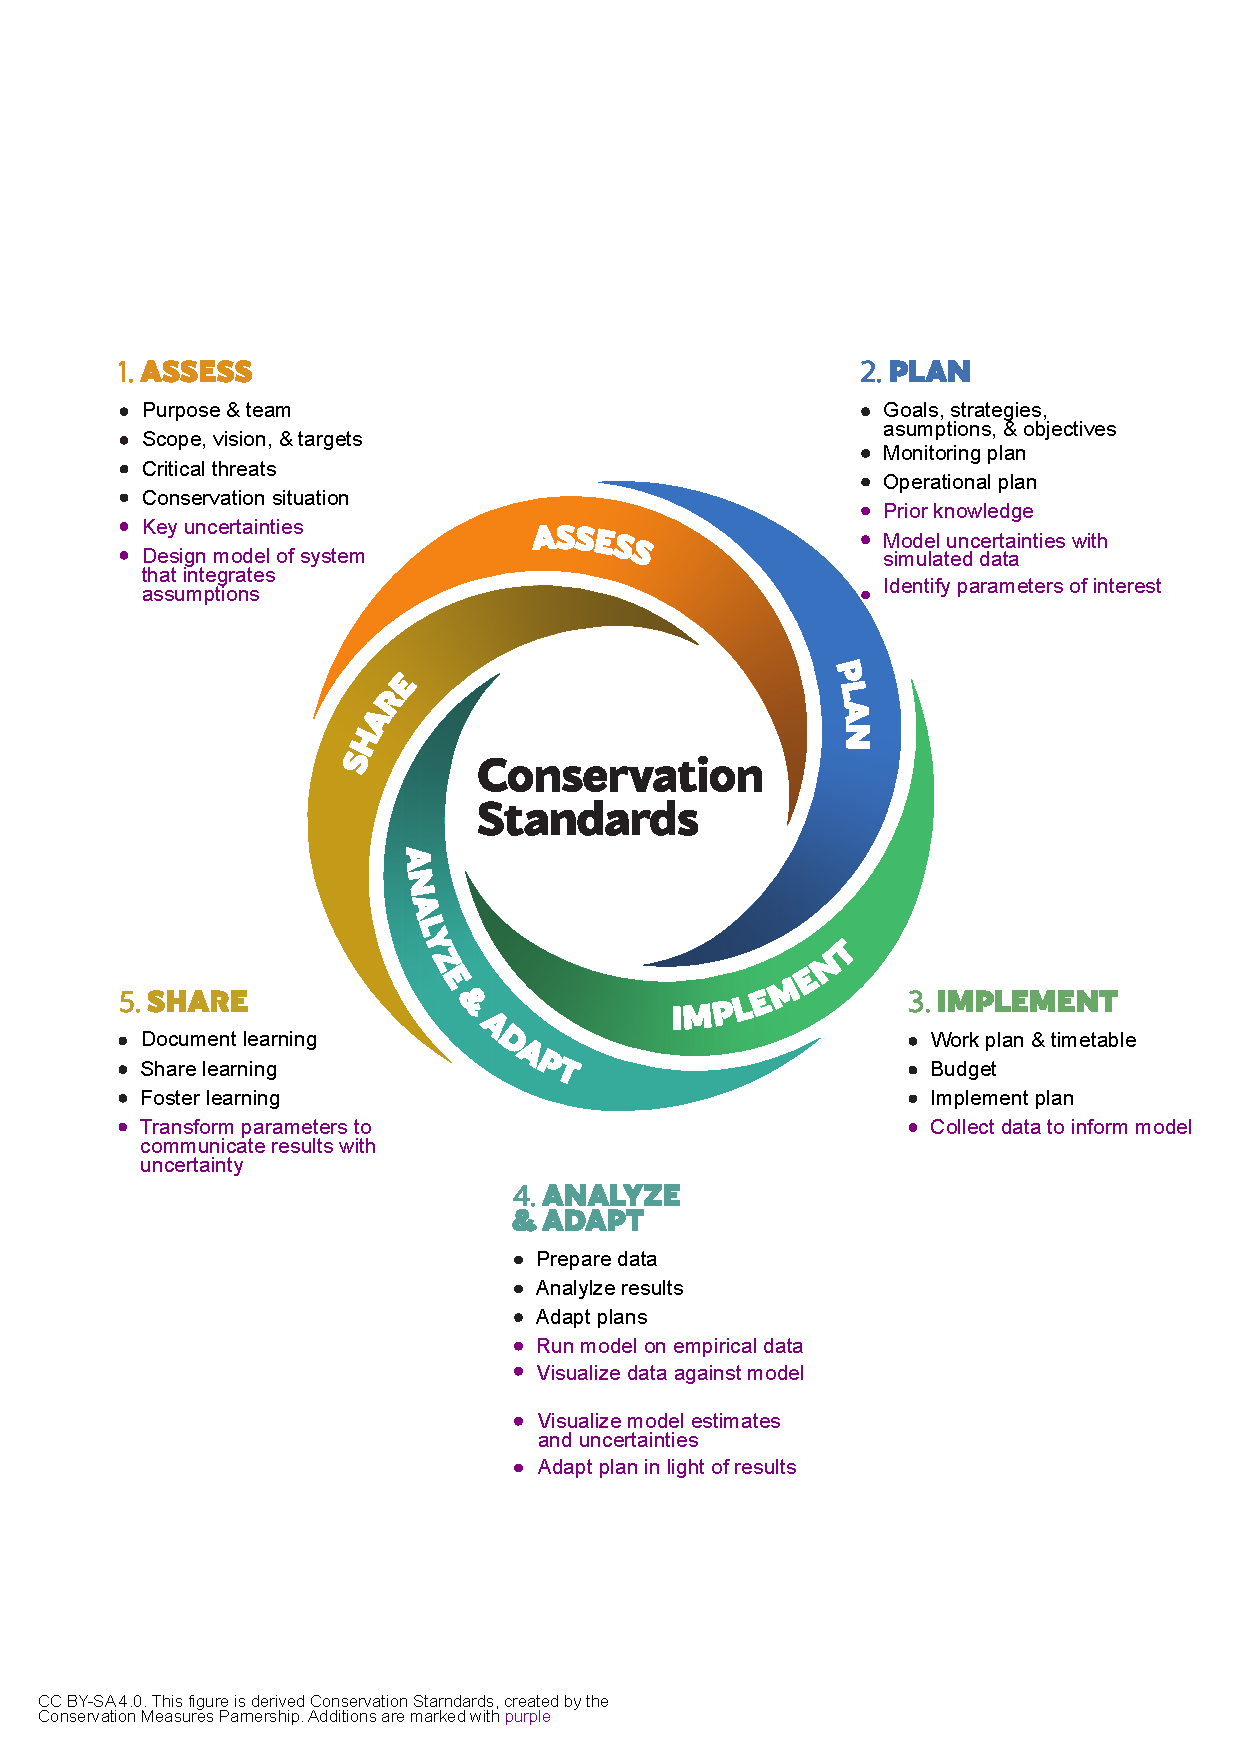
\includegraphics[width=0.75\textwidth]{../figs/CS_revised.pdf}
 \caption{\textbf{The iterative nature of Bayesian workflows aligns well with cycles of adaptive management in conservation}. Integrating analytical approaches through cyclical stages of conservation planning and implementation-- rather than only in one later stage-- is likely to lead to better planning and implementation outcomes.} 
 \label{fig:workflow}
 \end{figure}


\begin{figure}[h]
\centering
 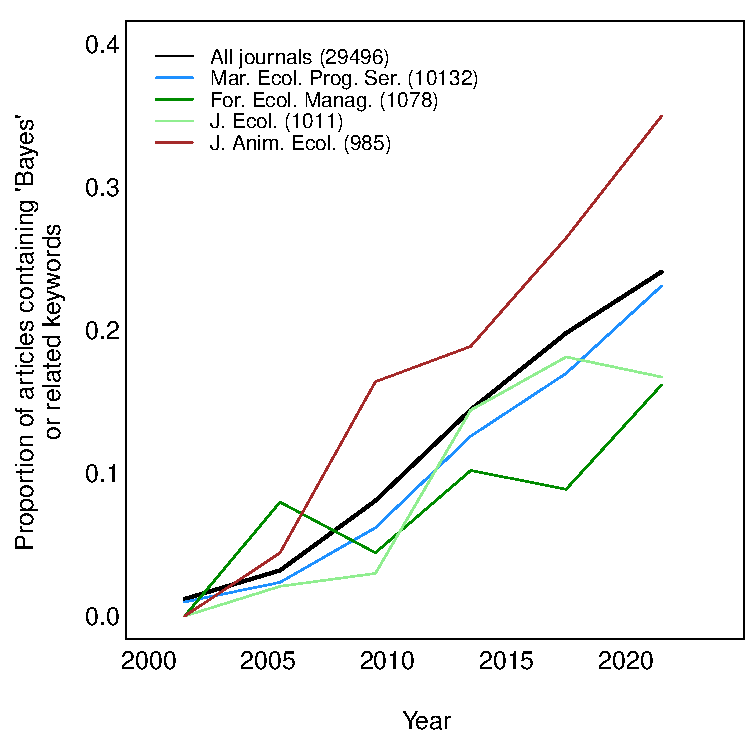
\includegraphics{../figs/conservation.pdf}
 \caption{\textbf{Proportion papers using Bayes in XX major conservation journals since 2000}}
 \label{fig:consbaystrend}
 \end{figure}

%DLJuly30: Still needs an explanation that dashed lines are included for populations with significant growth over time and that in b the points depict the mean change in abundance for each population's posterior estimates and the bars the 90\% uncertainty interval. 
\begin{figure}
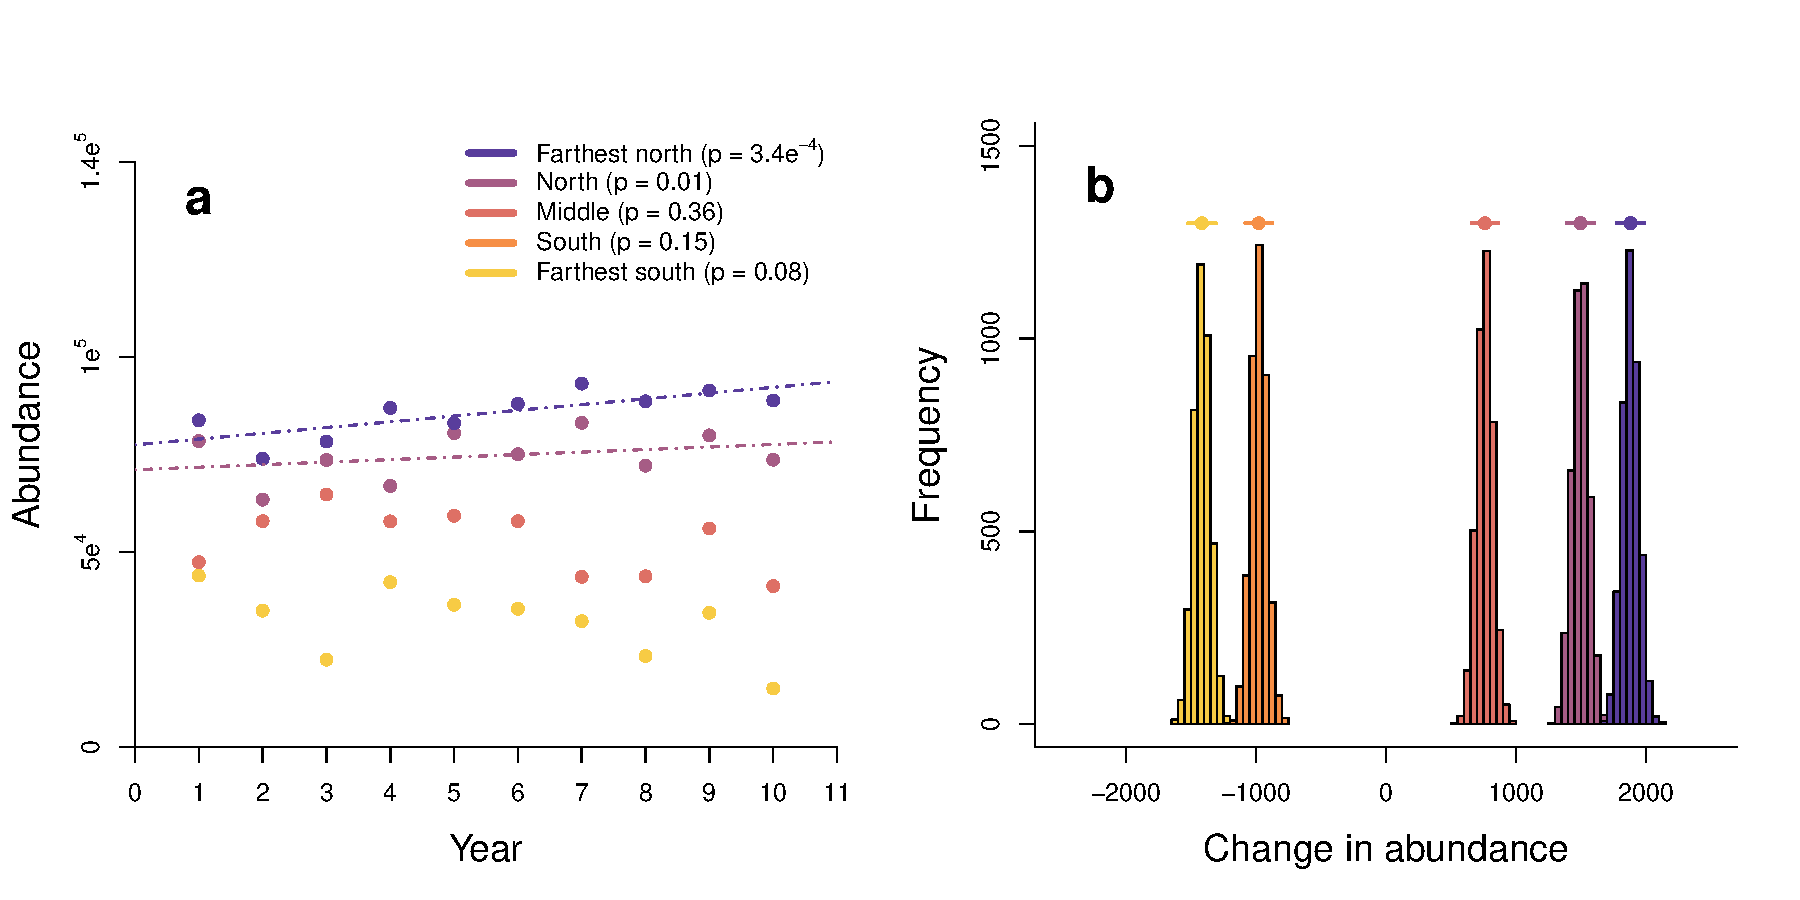
\includegraphics[width=1\textwidth]{../bayesvfisherbox/figures/nhtBoxLayeredMeans.pdf}
\caption{Trends in population size over time (left) analyzed with a traditional Fisherian approach using null hypothesis testing (using an $\alpha$ of 0.05 to reject the null hypothesis of a slope of zero) versus a Bayesian approach, which focuses on the posterior distribution (right).}
\label{fig:nht}
\end{figure}
  %DLJuly30: I would jitter the points to better see the two sets of error
  
 \begin{figure}[h]
\centering
 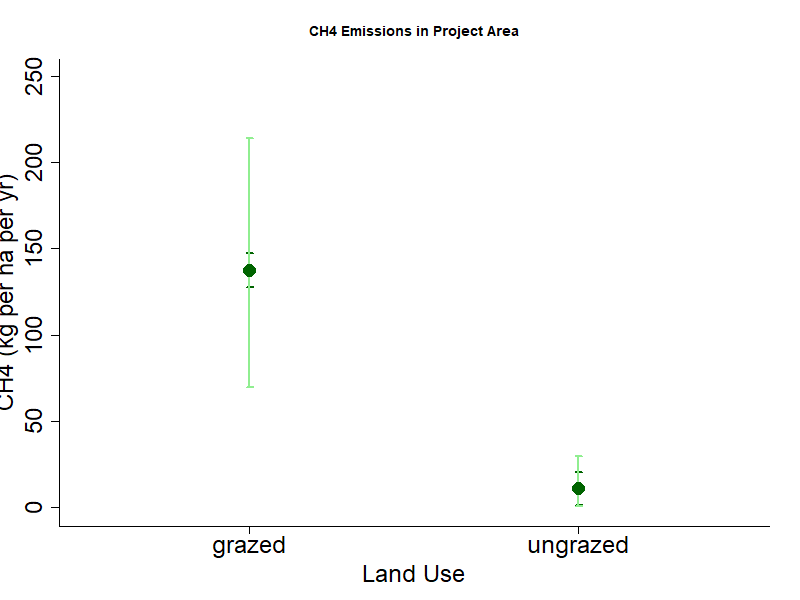
\includegraphics{../figs/ncs/ncsprojimpactch4.png}
 \caption{\textbf{NCS Example: Uncertainty propagation}} 
 \label{fig:ncs}
 \end{figure}
 
 

%%%%%%%%%%%%%%%%%%
%%%%%%%%%%%%%%%%%%%%%%
\end{document}
%%%%%%%%%%%%%%%%%%%%%%%%%%%%%%%%%%%%%%%%
% and for Nationally Determined Contributions, National Adaptation Plans, and other climate plans within the United Nations climate process are informed by the 'best available science.'
%Questions for the group:
%1) How detailed to get in Bayesian methods/theory in introduction?

%Text to add somewhere:
% in the past, climate science and biodiversity fields have been separated, but scientists and decision-makers  are increasingly highlighting  the role nature plays in global climate systems and the critical ecosystem services provided by nature to humans \citep{cohen2016nature,nesshover2017science,USGCRP2024}

